%% load necessary packages
\documentclass[paper=a4, fontsize=11pt,parskip=half,headings=small]{scrartcl}
\usepackage{check-short}
\usepackage{overpic}
\usepackage{multirow}


%% set author information etc
\title{Some title}
\author{Constantin Heck, Erlend Hodneland, Erik A. Hanson, \\ Arvid Lundervold, Jan Modersitzki, Alexandre Malyshev \\ (random order)}
\date{\today}


%% define some local commands
\newcommand{\Qso}{Q_{\mathrm{so}}}
\newcommand{\Qsi}{Q_{\mathrm{si}}}
\newcommand{\ca}{c_\mathrm{a}}
\newcommand{\CBV}{\mathrm{CBV}}
\newcommand{\MTT}{\mathrm{MTT}}
\newcommand{\cout}{c_{\mathrm{v}}}
\newcommand{\Pa}{P_{\mathrm{a}}}
\newcommand{\Pout}{P_{\mathrm{v}}}


%define SI-units, since we want to be able to easily change them
\newcommand{\siq}{\cubic\milli\meter\per\second\per\square\milli\meter}
\newcommand{\siqt}{\cubic\milli\meter\per\second}
\newcommand{\siP}{\cubic\milli\meter\per\second\per\cubic\milli\meter}
\newcommand{\siQ}{\kilo\gram\per\second\per\cubic\milli\meter}
\newcommand{\sirho}{\kilo\gram\per\cubic\milli\meter}
\newcommand{\siJ}{\milli\mol\per\second\per\square\milli\meter}
\newcommand{\sic}{\milli\mol\per\cubic\milli\meter}
\newcommand{\siPn}{\milli\litre\per\minute\per100\milli\litre}

%define misc commands
\newcommand{\missingsource}{\textcolor{red}{[?]}}

%--------------------------------------------------------------------------------------------
%--------------------------------------------------------------------------------------------
% Here begins the document, remove "draft" option in document class to include images
%--------------------------------------------------------------------------------------------
%--------------------------------------------------------------------------------------------
\begin{document}
	%--------------------------------------------------
	% Title Page=
	%--------------------------------------------------
	\maketitle
	\tableofcontents
	
	
	
	%--------------------------------------------------
	%--------------------------------------------------
	% Section: Classical models
	%--------------------------------------------------
	%--------------------------------------------------
	\section{Classical Models} \label{sec:classical}

	We will first describe two standard models to recover CBF,CBV and MTT from data displaying propagation of a contrast agent through the tissue.
	The so-called Deconvolution Model (DM) is used in vast amount of publications \cite{ostergaard96,abels10,straka10,bivard13,sourbron13} and has been shown to yield accurate parameter results.
	However, the application of the algorithm to real data is still challenging as it is sensitive to noise and to patient movement \cite{kudo10}.
	Another model which has been shown to exhibit good properties in restoring CBF and MTT is the so-called Maximum Slope Model (MS) \cite{miles91,klotz99}.
	The maximum slope model has been shown to exhibit advantages over the deconvolution model especially if uptake curves are degraded in the late phase \cite{abels10}.
		
	We now briefly present the theoretical basis of two models \cite{sourbron13}.
	Let $\Omega_i$ be a control volume with one inlet and one outlet and let $C(t)$ denote the CA concentration within $\Omega_i$ at timepoint $t$.
	Let us furthermore assume linearity and stationarity of CA in- and outflow with proportionality constants $\Pa,\Pout$ \si{\siP}.
	These assumptions lead to the differential equation 
	\begin{equation}
		C'(t) = \Pa\ca(t) - \Pout\cout(t)
		\label{eq:classicgeneral}
	\end{equation}
	where $\ca,\cout$ are the CA concentrations at the inlet and outlet of $\Omega_i$. 	
	In the next step, the deconvolution model and the maximum slope model are making different assumptions

	%----------------------------------------------------------
	% Subsection: The Convolution Model: Theory and Implementation
	%----------------------------------------------------------	
	\subsection{The Convolution Model: Theory and Implementation}\label{sec:conv}
	
	For the deconvolution model it is assumed that there is a probability distribution describing transit times $h(t)$ through $\Omega_i$. 
	The conservation of mass argument leads to
	\[
		\Pout\cout(t) = (h*\Pa\ca)(t) := \Pa\int_0^t \ca(s) h(t-s) \diffint s.
	\]
	Combining this with \eqref{eq:classicgeneral} yields $C'(t) = \Pa\ca(t)-\Pa (h*\ca)(t)$.
	Integrating the latter equation and using basic properties of the convolution one obtains
	\begin{equation}
		C(t) = (I*\ca)(t)
		\label{eq:conv}
	\end{equation}
	for the impuls-response function $I(t) := \Pa(1-\int_0^t h(s) \diffint s)$.
	One can show that $I$ fulfills the following properties:
	\begin{itemize}
		\item $I(0) = \Pa$,
		\item $I$ is monotonously decreasing,
		\item $I\ge 0$.		
	\end{itemize}
	The problem to identify $I$ given a tissue curve $C$ and an arterial input function $\ca$ is a deconvolution problem.
	If $I$ is recovered, $\Pa$ can subsequently be estimated as $\Pa = \max_{t} I(t)$.
	There are several methods to perform the deconvolution.
	A standard approach using Fourier-based algorithms has been shown sensitivity in the presence of noise \cite{wirestam00,ostergaard96}.
	Another class of deconvolution algorithms gaining increasing attention are based on Bayesian modeling \cite{boutelier12,mouridsen06}.
	Recent evaluations are showing good performance \cite{sasaki13}, however the numerical handling is difficult complex numerical integrations have to be performed.
	The class most popular among deconvolution algorithms is based on singular value decomposition (SVD) \cite{ostergaard96}.
	These algorithms have been shown to be quite robust in the presence of noise.
	Also, they can be easily adapted to be robust against large delays in tracer arrival using block-circular structures (bSVD cf. \cite{wu03}).
	In order to identify the impuls-response functions $I$ from the simulated data, we hence decided to use the bSVD model as proposed in \cite{wu03}.

	%----------------------------------------------------------
	% Subsection: A Second Digital Phantom For Validation
	%----------------------------------------------------------	
	\subsection{The Convolution Model for a Well-Mixed Compartment} \label{sec:comp}
	Let us assume that $\Omega_i$ is a well-mixed compartment where $C(t) = \phi\cout(t)$ for some $0 < \phi \le 1$ and that additionally $\Pout=\Pa$.
	In this case \eqref{eq:classicgeneral} reduces to
	\begin{align*}
		(\phi \cout)' &= \Pa \ca - \Pa \cout, \\
		\cout(0)&=0.
	\end{align*}
	Letting $\MTT:=\Pa/\CBV$ yields the solution
	\[
		C(t) = \Pa \int_0^t e^{-1/\MTT(t-s)}\ca(s)\diffint s
	\]
	with residue function $R(t)=e^{-t/\MTT}$. 

	
	
	
	%----------------------------------------------------------
	% Subsection: The Maximum Slope Model
	%----------------------------------------------------------
	\subsection{The Maximum Slope Model: Theory and Implementation}\label{sec:ms}	
	In the MS Model, equation \eqref{eq:classicgeneral} is combined with the assumption that $\Pout = \Pa$ (cf. \cite{klotz99}).
	This yields:
	\[
		\Pa = \frac{C'(t)}{\ca(t) - c_v(t)}.
	\]
	Assuming that $t$ is in an early uptake-phase where no contrast agent is leaving the system yet, it holds approximately that
	\[
		\Pa = \frac{C'(t)}{\ca(t)} \iff P\ca(t) = C'(t).
	\]
	Differentiating this equation with respect to $t$ yields:
	\[
		\Pa \ca'(t) = C''(t).
	\]
	Assuming that if $\ca$ peaks there is no or only a negligible amount of CA leaving the system, this equation is also fulfilled for timepoint $t_{\mathrm max}:=\mathrm{argmax}_{t}\ca(t)$. 
	Since at this point it holds that $\ca'(t_{\mathrm max}) = 0$ and hence also $C''(t_{\mathrm max})=0$, we derive
	\begin{equation}\label{eq:MS}
		\Pa = \frac{\max_{t}C'(t)}{\max_{t}\ca(t)}.
	\end{equation}
	
	
	
	
	
	
	
	
	%--------------------------------------------------
	%--------------------------------------------------
	% Section: The synthetic model
	%--------------------------------------------------
	%--------------------------------------------------	
	\section{The Novel Synthetic Model}\label{sec:synthetic}
	
	Structurally, the model-assumptions for both classical methods presented in Section \ref{sec:classical} are similar.
	Both are assuming that the region of interest where the model is applied exhibits only one inlet and one outlet.
	In fact, this assumption is questionable when we describe CA propagation through a larger area with a highly developed capillary system.
	Here we expect in contrast a coupled systems, since each voxel can be regarded as an inlet for the surrounding voxels.
	We hence decided to describe the CA propagation as a spatially coupled transport process. 
	Details of the modeling of transport will be presented in Section \ref{sec:transport}.	
	
	Since the CA transport itself is driven mainly by blood flow, we will describe a simple model for the blood flow through capillary tissue in Section \ref{sec:flow}.
	Within the capillary system we expect the blood flow to be driven mainly by differences in pressure.
	This way of modeling flow comes from the theory of porous media and is expressed in Darcy's law \missingsource.
	As a consequence, we will also apply the physical understanding of flow as surface flux $q = q(x)$ with units \si{\siq}.
	The surface flux is a vector field describing the volume of fluid per unit time flowing across a sliced unit area of the sample.	
	However, a model to convert surface flux to perfusion with units \si{\siP} will be introduced in Section \ref{sec:flux2perf}.
	The resulting CA flux $J(x,t)$ with units \si{\siJ} is assumed to be linear and stationary, meaning that $J(x,t) = q(x)\cdot c(x,t)$.
	Apart from the normalization with respect to surface, the assumptions of linearity and stationarity are in complete agreement with standard pharmacokinetic modeling \cite{sourbron13}.
	A detailed description of modeling the blood flow can be found in Section \ref{sec:flow}.
	
	Another key ingredient from porous media is the introduction of the porosity $\phi$ for $0 \le \phi \le 1$.
	The porosity describes which fraction of a small tissue volume is accessible for blood.
	Comparing with pharmacokinetic modeling, the porosity directly translates to the cerebral blood volume (CBV).
	
	We will now describe the construction of the digital phantom in detail.	
	
	%--------------------------------------------------
	% Subsection: Modeling the Blood Flow
	%--------------------------------------------------
	\subsection{Modeling the Blood Flow}\label{sec:flow}
	
	We model the blood flow as the flow of a fluid through a porous medium. 
	The fluid has units \si{\sirho} and is denoted by $\rho = \rho(x,t)$.
	As explained previously, the flux $q$ (in \si{\siq}) as well as the porosity $\phi$ (with $0 \le \phi \le 1$) are assumed to be stationary and hence independent of time.
	Fluid introduced and extracted from the system is modeled by a source- and sink term $\tilde{Q} = \tilde{Q}(x)$ with units \si{\siQ}. 
	The continuity equation describing conservation of mass now states that
	\begin{equation}
		\frac{\partial (\phi \rho)}{\partial t} + \nabla \cdot (\rho q) = \tilde{Q}.
		\label{eq:syntcont}
	\end{equation} 
	Furthermore assuming that the system is in steady-state and that the density of blood $\rho(x)$ is constant in space, we obtain that $\diffopcal{\rho}{t} = 0$ and hence:
	\begin{equation}
		\nabla \cdot q = \frac{\tilde{Q}}{\rho}.
		\label{eq:syntcontsimp}
	\end{equation}
	In order to scale away the density $\rho$ we define another source term $Q$ with units \si{\siQ} having the relation $Q := \tilde{Q}\rho$, thus transforming \eqref{eq:syntcontsimp} into
	\begin{equation}
		\nabla \cdot q = Q.
		\label{eq:syntcontsimp2}
	\end{equation}
	The right hand side is only non-zero within the source or the sink. 
	Elsewhere, \eqref{eq:syntcontsimp2} is concurrent with the incompressibility condition of divergence free flow.
	
	Low velocity fluid flux in porous media is described by Darcy's law \missingsource:
	\[
		q = -\frac{K}{\mu} \left( \nabla p + \rho g  \nabla z \right).
	\]
	here $g$ is the gravitational acceleration, $K$ is the permeability tensor with units \si{\square\milli\meter}, $z$ is the spatial position along the gravitational field and $\mu = \mu(x)$ is the viscosity of the fluid with units $\si{\pascal\second}$.
	For the current project the flux is taking place perpendicular to the gravitational field and the gravitational term can thereby be discarded.
	That a simplified version of Darcy's law thus becomes
	\begin{equation}
		q = -\frac{K}{\mu} \nabla p.
		\label{eq:syntdarcysimp}
	\end{equation}
	We now combine \eqref{eq:syntcontsimp2} and \eqref{eq:syntdarcysimp} and assume that $K$ is symmetric and positive definite.
	This yields the following elliptic partial differential equation the pressure-field $p$ with units \si{\pascal} must fulfill:
	\begin{equation}
		\left\vert
		\begin{alignedat}{2}
			\nabla \cdot \left( -\frac{K}{\mu} \nabla p \right) &= Q  \qquad &&x \in \Omega, \\
			n \cdot \nabla p &=0 &&x \in \partial \Omega.
		\end{alignedat}
		\right\vert
		\label{eq:flowmodel}
	\end{equation}
	Here $\partial \Omega$ denotes the boundary of $\Omega$ and $n$ the outward unit normal vector. 
	Modeling an isolated system with no inflow or outflow along the boundary of $\Omega$, we impose the Neumann boundary conditions $n \cdot \nabla p = 0$ on $\partial \Omega$.
	Note that \eqref{eq:flowmodel} exhibits a solution which unique up to constant since only pressure differences are taken into consideration \cite{evans98}.
	Having solved \eqref{eq:flowmodel} the flux field can be computed according to \eqref{eq:syntdarcysimp} from the obtained pressure map. 
	
	
	%--------------------------------------------------
	% Subsection: Modeling the Contrast Agent Transport
	%--------------------------------------------------	
	\subsection{Modeling the Contrast Agent Transport}\label{sec:transport}
	In this section we will describe how the CA propagates in the tissue according to the flow-field.
	We assume that the CA is introduced at a source- and extracted at a sink location.
	The concentration map resulting from the simulation is later used to model the CA concentration one would observe with MRI or CT measurements.
	
	In order to define meaningful continuous contrast agent concentrations, we first describe the CA concentration in an (arbitrarily) small tissue volume $\Omega_i$.
	Assume that $V_i$ is the volume of $\Omega_i$ and $v_i$ the the blood volume of $\Omega_i$.
	By definition the porosity is in this case given by $\phi_i = v_i/V_i$.
	Let $C_i(t)$ denote the CA concentration in $\Omega_i$ with respect to the whole volume $V_i$ at timepoint $t$.
	The CA concentration with respect to the blood volume $v_i$ will be denoted by $c_i(t)$.
	Both concentrations have units \si{\sic}. 
	From the definition of $c_i,C_i$ and $\phi_i$ we obtain the relation $C_i = \phi_i \cdot c_i$.

	The rate of change of tracer molecules within the control volume $\Omega_i$ can he described by
	\begin{equation}
		\diffop{t}\int_{\Omega_i}C_i \diffint x = \int_{\Omega_i}\diffop{t}(\phi_i c_i) \diffint x.
		\label{eq:dmdt}
	\end{equation}	
	Since we expect mainly transport along the vessels and marginal diffusion, the change in tracer mass within $\Omega_i$ occurs only from advective flow and the source and sink field $Q$.
	Let us write the source- and the sink term as $Q = \Qsi + \Qso$ where $\Qsi \le 0$ is the sink and $\Qso \ge 0$ is the source. 
	Both are assumed to be zero everywhere except at in the respective source and sink locations.
	Note that $Q = \Qso + \Qsi$ and $\int_\Omega Q \diffint x = 0$ in line with incompressible flow. 
	The change in contrast agent at time point $t$ can hence be written as
	\begin{equation}
		-\int_{ \Gamma_i}c_i(q_i \cdot n)\diffint s + \int_{\Omega_i}\ca \Qso \diffint x + \int_{\Omega_i}c_i\Qsi \diffint x,
		\label{eq:surfflux}
	\end{equation}
	where $n$ is the outward unit normal on $\Gamma_i := \partial \Omega_i$.
	Furthermore $\ca = \ca(t)$ with unit \si{\sic} describes the amount of contrast agent entering the system at the source. 
	In standard pharmacokinetic modeling, $\ca$ is referred to as the arterial input function (AIF).
	From preservation of the tracer mass, equations \eqref{eq:dmdt} and \eqref{eq:surfflux} must balance such that
	\begin{equation}
		\int_{\Omega_i}\diffop{t} (\phi_i c_i) \diffint x + \int_{ \Gamma_i}c_i(q_i \cdot n) \diffint s = \int_{\Omega_i}\ca\Qso \diffint x + \int_{\Omega_i}c \Qsi \diffint x.
		\label{eq:conteq}
	\end{equation}
	Upon application of the divergence theorem, \eqref{eq:conteq} is consistent with the continuity equation on local form
	\begin{equation}
		\left\vert
		\begin{alignedat}{2}
			\phi \frac{\partial c}{\partial t} + \nabla \cdot (cq) &= \ca\Qso + c\Qsi \qquad	&x &\in \Omega, \ t>0,  \\
			c &= 0 																			 	&x &\in \Omega, \ t=0.
		\end{alignedat}
		\right\vert
		\label{eq:conteqlocal}
	\end{equation}
	This is a linear transport equation in $c(x,t)$. 
	Assuming that $\phi$ is Lipschitz continuous and that $\Qso,\Qsi,\ca$ are continuous, we can follow that $q$ is as the solution of \eqref{eq:flowmodel} also Lipschitz continuous.
	In this case we can follow \cite{evans98} to see that \eqref{eq:conteqlocal} exhibits a unique local solution.
	


	%--------------------------------------------------
	%--------------------------------------------------
	% Section: Relating the classical and the synthetic model
	%--------------------------------------------------
	%--------------------------------------------------	
	\section{Relating the Classical and the Synthetic Model}\label{sec:relation}
	Here is still some motivation missing.
	
	In order to test the standard models for their abilities to restore CBF and CBV, we need to convert the flux $q$ with units \si{\siq} to perfusion $P$ with units \si{\siP}. 
	A method to do that will be presented in Section \ref{sec:flux2perf}.
	In Section \ref{sec:CBV} we will give a proof that the porosity CBV can be estimated from the standard relationship $\CBV = \left(\int_0^\infty C(x,s) \diffint s\right)/\left(\int_0^\infty \ca(s) \diffint s\right)$.
	
	
	
	%--------------------------------------------------
	% Subsection: Converting Flow to Perfusion
	%--------------------------------------------------
	\subsection{Converting Flow to Perfusion}\label{sec:flux2perf}
	The model described in \eqref{eq:flowmodel} uniquely determines the flux field $q(x)$. 
	However, in pharmacokinetic modeling the parameter of interest is usually the cerebral blood flow (CBF), which we will denote by $P(x)$.
	It is not obvious how to transform a flux field into a scalar perfusion field $P(x)$.
	There are at least two obvious differences between $q$ and $P$. 
	First, the flux is a vector field and the perfusion is a scalar field. 
	Second, the flux relates to a surface area and the perfusion relates to a volume. 
	Thus, these to quantities are strictly, mathematically different but still conceptually related. 
	In the following we describe a method for converting flux into perfusion.

	The classical understanding of perfusion is the amount of blood feeding a tissue volume per unit time. 
	Thus, the perfusion $P$ has the units \si{\siP}.
	It is common to scale this quantity to normalized perfusion $P_n(x)$ with units \si{\siPn}. 
	One approach for converting flux into perfusion could be to estimate the perfusion as the total inflow (or outflow) of fluid (e.g. arterial blood) into a control region per unit time, and then normalizing with the control region volume. 
	This is only a valid approach if every control region is separated from other control regions, and not feeding each other. 
	Thus, this approach is valid for an entire organ being the control region. 
	Such understanding is in line with the understanding of classical compartment models for perfusion where each voxel has its own source of feeding arterial blood, independent of the neighbor voxels. 
	Clearly, this is a simplification since voxels will be fed by their neighbors. 
	In our synthetic flow model SFM as well as in normal tissue this assumption is violated since the voxels are feeding their neighbor voxels with arterial blood. 
	Simply summing the total inflow into a voxel and dividing by the voxel volume will strongly over-estimate the perfusion since we would divide by the wrong normalization volume. 
	The problematic issue is that the incoming blood is feeding more voxels than the current voxel. 
	This phenomenon is demonstrated in Fig. \ref{fig:perfusion-problem} where the volume on the left has the true perfusion value of $P_1 = F_0/(2V)$ for an incoming flow $F_0$ in \si{\siqt} and distribution volume $2V$ in \si{\cubic\milli\meter}. 
	However, for another discretization as shown in the middle, the perfusion within each of these sub-volumes becomes $P_2 = F_0/V = 2P_1$. 
	Taking the average across both sub-volumes, it is clear that the perfusion is over-estimated with a factor of two. 
	A discretization dependent perfusion value is not desirable, and the perfusion estimate of $P_2$ is clearly wrong. 


	\begin{figure}[H]
	    \centering
	    \begin{overpic}[scale=0.5]{figs/perfusion-problem.eps}
	    	\put(11,67){\color{black}$F_0$}
			\put(49,67){\color{black}$F_0$}
			\put(85.2,66){\color{black}$\Delta F_0$}
			\put(13,33){\color{black}$2V$}
			\put(50,20){\color{black}$V$}
			\put(50,45){\color{black}$V$}
			\put(91,42){\color{black}$\Delta V$}
		\end{overpic}
	    \caption{Perfusion within a small volume. Left: A compartment with volume $2V$ is exposed to a flow $F_0$ $\si{\siqt}$ of fluid. From definition, the overall perfusion within this object becomes $P_1 = F_0/(2V)$ \si{\siq}. Right: The volume is divided into two smaller compartment (e.g. voxels), and the perfusion for each of the compartments becomes $P_2 = F_0/V = 2P_1$. This discrepancy between the two discretisation regimes occurs because the flow is counted twice as it is fed from one voxel to the other. Right: As a solution to the described problem we pick out a true distribution volume $\Delta V$ (area in this 2D sketch), which is a small area around a given streamline along the centre line of the grey area. This is the true distribution volume (area) which is feeded with arterial blood from the incoming fractional flow $\Delta F_0$. The correct perfusion within $\Delta V$ is therefore $\Delta F_0/dV$. The entire compartment can further be divided into infinitesimal distribution volumes, thus providing voxelwise perfusion values.}
	    \label{fig:perfusion-problem}
	\end{figure}

	The reason for this discrepancy is that for $P_2$ the perfusion has been counted twice since we are dividing by the wrong distribution volume. 
	Instead, we need to consider to the classical definition of perfusion. 
	The concept of perfusion has a very precise meaning, as the amount of arterial blood per time unit delivered to a capillary bed in a biological tissue, and then scaled by the feeded tissue volume. 
	Therefore, we must divide the incoming flow by the total distribution volume that is covered by the fluid streamlines. 
	This formulation coincides with the classical understanding of perfusion, and the correct distribution volume will rather be the volume that the fluid particles within an infinitesimal cross-sectional area around the streamlines are covering. 
	Assuming laminar flow, the streamlines are not crossing each other and we can estimate the true distribution volume that is fed by a given arterial blood flow.

	Let us fix a point $y \in \Omega$.
	Formally, the direction of the streamline passing $y$ is identical to the flux $q(y)$ at this location. 
	Let $A_\varepsilon$ be a 2-D disc with radius $\varepsilon$ which is orthogonal to $q(y)$.
	The total flow of particles \si{\siqt} over the disc can be expressed as
	\[
		F = \int_{A_\varepsilon} (q \cdot n) \diffint A = \int_{A_\varepsilon} \left(q\cdot \frac{q(y)}{\Vert q(y) \Vert}\right) \diffint A.
	\]
	Let $l \subset \Omega$ be the (unique) streamline passing through $y$ and let $L$ denote be the length of $l$.
	We now consider a small tube $T$ of radius $\varepsilon$ around $l$.
	Following Cavalieri's principle the volume $V$ of $T$ can be expressed as $V = \varepsilon^2\pi L$
	Hence we can express the perfusion $P_\varepsilon$ for this volume as
	\[
		P_\varepsilon = \frac{F}{V} = \frac{1}{\varepsilon^2 \pi L} \int_{A_\varepsilon} \left( q\cdot \frac{q(y)}{\Vert q(y) \Vert} \right) \diffint A. 
	\]
	Letting $\varepsilon \to 0$ and using that $F/(\varepsilon^2\pi)$ goes to $\Vert q(y) \Vert$ if $q(x)$ is continuous yields a value for the perfusion $P_{y}$:
	\begin{equation}
		P_{y} = \frac{\Vert q(y) \Vert}{L}
		\label{eq:flux2perf}
	\end{equation}
	where $L$ is the length of the streamline passing through the point $y$. 
	This is an explicit formula for converting flux into perfusion and is later used for evaluation of the classical model for perfusion. 
	
	
	


	%--------------------------------------------------
	% Subsection: Estimate the Porosity
	%--------------------------------------------------	
	\subsection{A Method to Estimate the Porosity}\label{sec:CBV}
	
	The principle of mass balance of fluid and tracer particles is described by \eqref{eq:flowmodel} and \eqref{eq:conteqlocal}. 
	For locations $x$ where $Q(x) = 0$ one can see that \eqref{eq:conteqlocal} becomes
	\[
		\phi\frac{\partial c}{\partial t}  = - q \cdot \nabla c.
		\label{eq:1cmodel}
	\]
	Integrating from $t_0$ to $t_1$ results in the model
	\[
		\phi [c(x,t_1) - c(x,t_0)]  = - \int_{t_0}^{t_1}q \cdot  \nabla c \diffint t.
	\]
	Going to the limit $t_0 = 0$ to $t_1 = \infty$, using the boundary conditions $c(x,0) = c(x,\infty) = 0$ and defining $E(x):= \int_0^\infty c(x,s) \diffint s$ leads to
	\[
		0 = q \cdot \nabla  E(x).
		\label{eq:streamlinezero}
	\]
	We can interpret this equation in such a way, that $q$ lies in-plane with the level-sets of the function $E(x)$.
	This means that $E(x)$ is constant along the streamlines of the fluid flow.
	Since we assumed that $Q$ has a delta-like structure and since all streamlines are emerging at the arterial-input, we obtain
	\[
		\int_0^\infty c(x,s) \diffint s = \int_0^\infty \ca(s) \diffint s.
	\]
	Using $C(x,t) = \phi(x) c(x,t)$ we obtain
	\begin{equation}
		\phi(x) =  \frac{ \int_{0}^{\infty} C(x,s) \diffint s }{ \int_{0}^{\infty} \ca(s) \diffint s}.
		\label{eq:phi}
	\end{equation}
	This expression coincides with the classical formula for CBV and is hereby proven analytically for the proposed model.
	
	
	
	

	%--------------------------------------------------
	%--------------------------------------------------
	% Section: Numerical implementation
	%--------------------------------------------------
	%--------------------------------------------------
	
	\section{Numerical Implementations}
	
	In this section we will describe how the model was implemented numerically.
	For simplicity we will assume that the domain is discretized by a regular cartesian grid of size $n \times n$ with a regular cell-spacing $h$.
	The proposed method may be extended for non-regular grids in an analogous fashion.
	
	Since conservation of mass is a key factor for both the discretization of the flow and the transport, we use algorithms preserve mass also in the simulations.
	To solve \eqref{eq:flowmodel} we used the two-point flux approximation finite volume method (TPFA) \missingsource. 
	Based on mass balance equations, we calculated the flux in such a fashion that conservation of mass was guaranteed.
	The transport equation \eqref{eq:conteqlocal} was solved by applying a straight-forward upwind scheme to \eqref{eq:conteq} \missingsource.

	%----------------------------------------------------------
	% Subsection: Discretization of the singe phase flow model
	%----------------------------------------------------------
	\subsection{Discretization of the Single Phase Flow Model using TPFA} \label{sec:numflow}

	We now shortly describe the direct application of the two-point flux approximation method \missingsource.
	Considering \eqref{eq:flowmodel} on a small domain (voxel) $\Omega_i \subset \Omega$ and applying the divergence theorem yields:
	\begin{equation}
		\int_{\partial \Omega_i}   -(\lambda \nabla p) \cdot \nu \diffint s = \int_{\Omega_i}Q \diffint x
	\label{eq:TPFAint}
	\end{equation}
	with conductivities $\lambda := K/\mu$.
	Defining $\Gamma_{i,j}$ as the boundary between neighboring voxels $\Omega_i$ and $\Omega_j$, one can see that mainly the component perpendicular to $\Gamma_{ij}$ will drive the flow between these voxels.
	The component of $\nabla p$ pointing along the normal vector of $\Gamma_{ij}$ can therefore be replaced in terms of the cell centered pressure values $p_i$ and $p_j$
 	$\Delta_h p_{ij} := \frac{(p_j - p_i)}{h}$, where $h$ denotes the grid-spacing.
	The total flux across the face $\Gamma_{ij}$ can hence be approximated by
	\[
		\Delta_h p_{ij} \int_{\Gamma_{ij}}\lambda \diffint s \approx (p_i - p_j) \underbrace{\frac{\lambda_{ij} \vert \Gamma_{ij} \vert}{h}}_{:=t_{ij}}.
	\]
	Here $|\Gamma_{ij}|$ is notation for the surface area of $\Gamma_{ij}$ and $\lambda_{ij}$ denotes an approximation of the mean conductivity on $\Gamma_{ij}$.
	The terms not depending on the pressure $p$ are collected into the transmissibilities $t_{ij}:=|\Gamma_{ij}|\lambda_{ij}/h$.
	Defining furthermore $F_i:=\int_{\Omega_i}Q\diffint x$ yields an approximation of \eqref{eq:TPFAint}, a linear system which can be solved for the pressure $p$ by a suitable solver.
	Note that $p,K$ and $\mu$ are assumed to be given cell-centered whereas the resulting flux is discretized on a staggered grid, corresponding to the voxel faces.


	%----------------------------------------------------------
	% Subsection: Discretization of the transport equation
	%----------------------------------------------------------
	\subsection{Discretization of the Transport Equation} \label{sec:numtrans}
	The transport described in \eqref{eq:conteq} was numerically implemented using an upwind Godunov scheme \missingsource.
	Let $c_i$ be a cell centered voxel tracer concentration and let $\Gamma_{ij}$ be the face between voxel $i$ and $j$ with outer unit normal $n_{ij}$.
	Let $q$ be the flux-field. 
	Then the total CA-flow over the face $\Gamma_{ij}$ can be estimated by
	\[
		\int_{\Gamma_ij} (c_i q)\cdot n_{ij} \diffint s \approx c_i q_{ij} \vert \Gamma_{ij} \vert.
	\]
	Keeping track of in- and outflow for each voxel and applying a straight-forward discretization of \eqref{eq:conteq} yields an explicit scheme to set up the transport simulation.
	A conversion of $c_i$ into $C_i$ is performed via the relation $C_i = c_i\phi_i$. 
	The overall concentration map $C_i$ is later used for the inverse problem of restoring CBV and CBF.





	%--------------------------------------------------
	%--------------------------------------------------
	% Section: Experiments
	%--------------------------------------------------
	%--------------------------------------------------
	\section{Experiments}\label{sec:NumExp}

	We will now describe the numerical experiments we performed.
	Based on \eqref{eq:flowmodel} and \eqref{eq:conteqlocal} we set up a forward simulation of blood-flow through the capillary system.
	A table of parameter values used for the numeral simulations are shown in Table \ref{tab:par}. 
	We aimed at creating a transparent synthetic test case and kept all optional parameters as simple as possible. 
	Therefore, the permeability and porosity were assumed constant in space and in time.
	The voxel-wise perfusion field $P$ was calculated according to $\eqref{eq:flux2perf}$. 
	The source term was chosen to the upper left voxel and the sink term was chosen in the lower right voxel.
	To model the arterial-input function, we chose a standard model \cite{wu03} given by the gamma function
	\[
		\ca(t) := t^\alpha e^{-t/\beta}
	\]
	for $\alpha=3$ and $\beta = \SI{1.5}{\second}$.
	
	\begin{table}[H]
		\centering
	  \caption{Parameters used in the numerical experiments, optimized for a slab of the capillary system in the human brain. In order to keep all parameters as simple as possible, permeability was assumed to be isotropic and permeability, porosity and viscosity were assumed constant.}		
		\begin{tabular}{ l  c  c  r }
		    Description 									& Symbol 			& Value(s) 				& Unit 				\\
			\toprule
		    Average input perfusion 				 		& $\overline{P}$ 	& $50$ 					& \si{\siPn}		\\
			Flow source, derived from $\overline{P}$ 		& $F_{so}$ 			& $0.08333$ 			& \si{\siqt}  		\\
			Flow sink 										& $F_{si}$ 			& $-F_{so}$ 		 	& \si{\siqt}  		\\
			Dynamic viscosity blood \cite{rosencranz06} 	& $\mu_b$ 			& $5 \cdot 10^{-6}$ 	& \si{\kilo\pascal\second}  	\\
			Fluid density blood \cite{kenner89} 			& $\rho$ 			& $1 $ 					& \si{\sirho} 		\\		
			Permeability  									& $k$ 				& $5 \cdot 10^{-6}$ 	& \si{\square\milli\meter} 			\\	
			Porosity\cite{wu03}								& $\phi$ 			& $0.05$ 				& \si{\cubic\milli\meter\per\cubic\milli\meter	}	\\	
			Spatial resolution 								& - 				& $(64,64,1)$ 			& -					\\
			Physical dimension 								& - 				& $(10,10,1)$ 			& \si{\milli\meter}				\\
			Voxel size 										& - 				& $(0.156,0.156,1)$ 	& \si{\milli\meter}	\\
	  \end{tabular}
	  \label{tab:par}
	\end{table}	
	
	In order to compare the Porous Media Model to the standard convolution model described in Section \ref{sec:conv}, an additional reference model was build.
	The reference model was set up assuming voxel-wise well-mixed compartments described in Section \ref{sec:comp} and the assumed perfusion values from \eqref{eq:flux2perf}.
	A comparison of the tissue curves at different positions of the tissue can be found in Figure \ref{fig:tissuecomp}. 



	\begin{figure}[H]
		\centering
            \begin{subfigure}[b]{0.3\textwidth}
				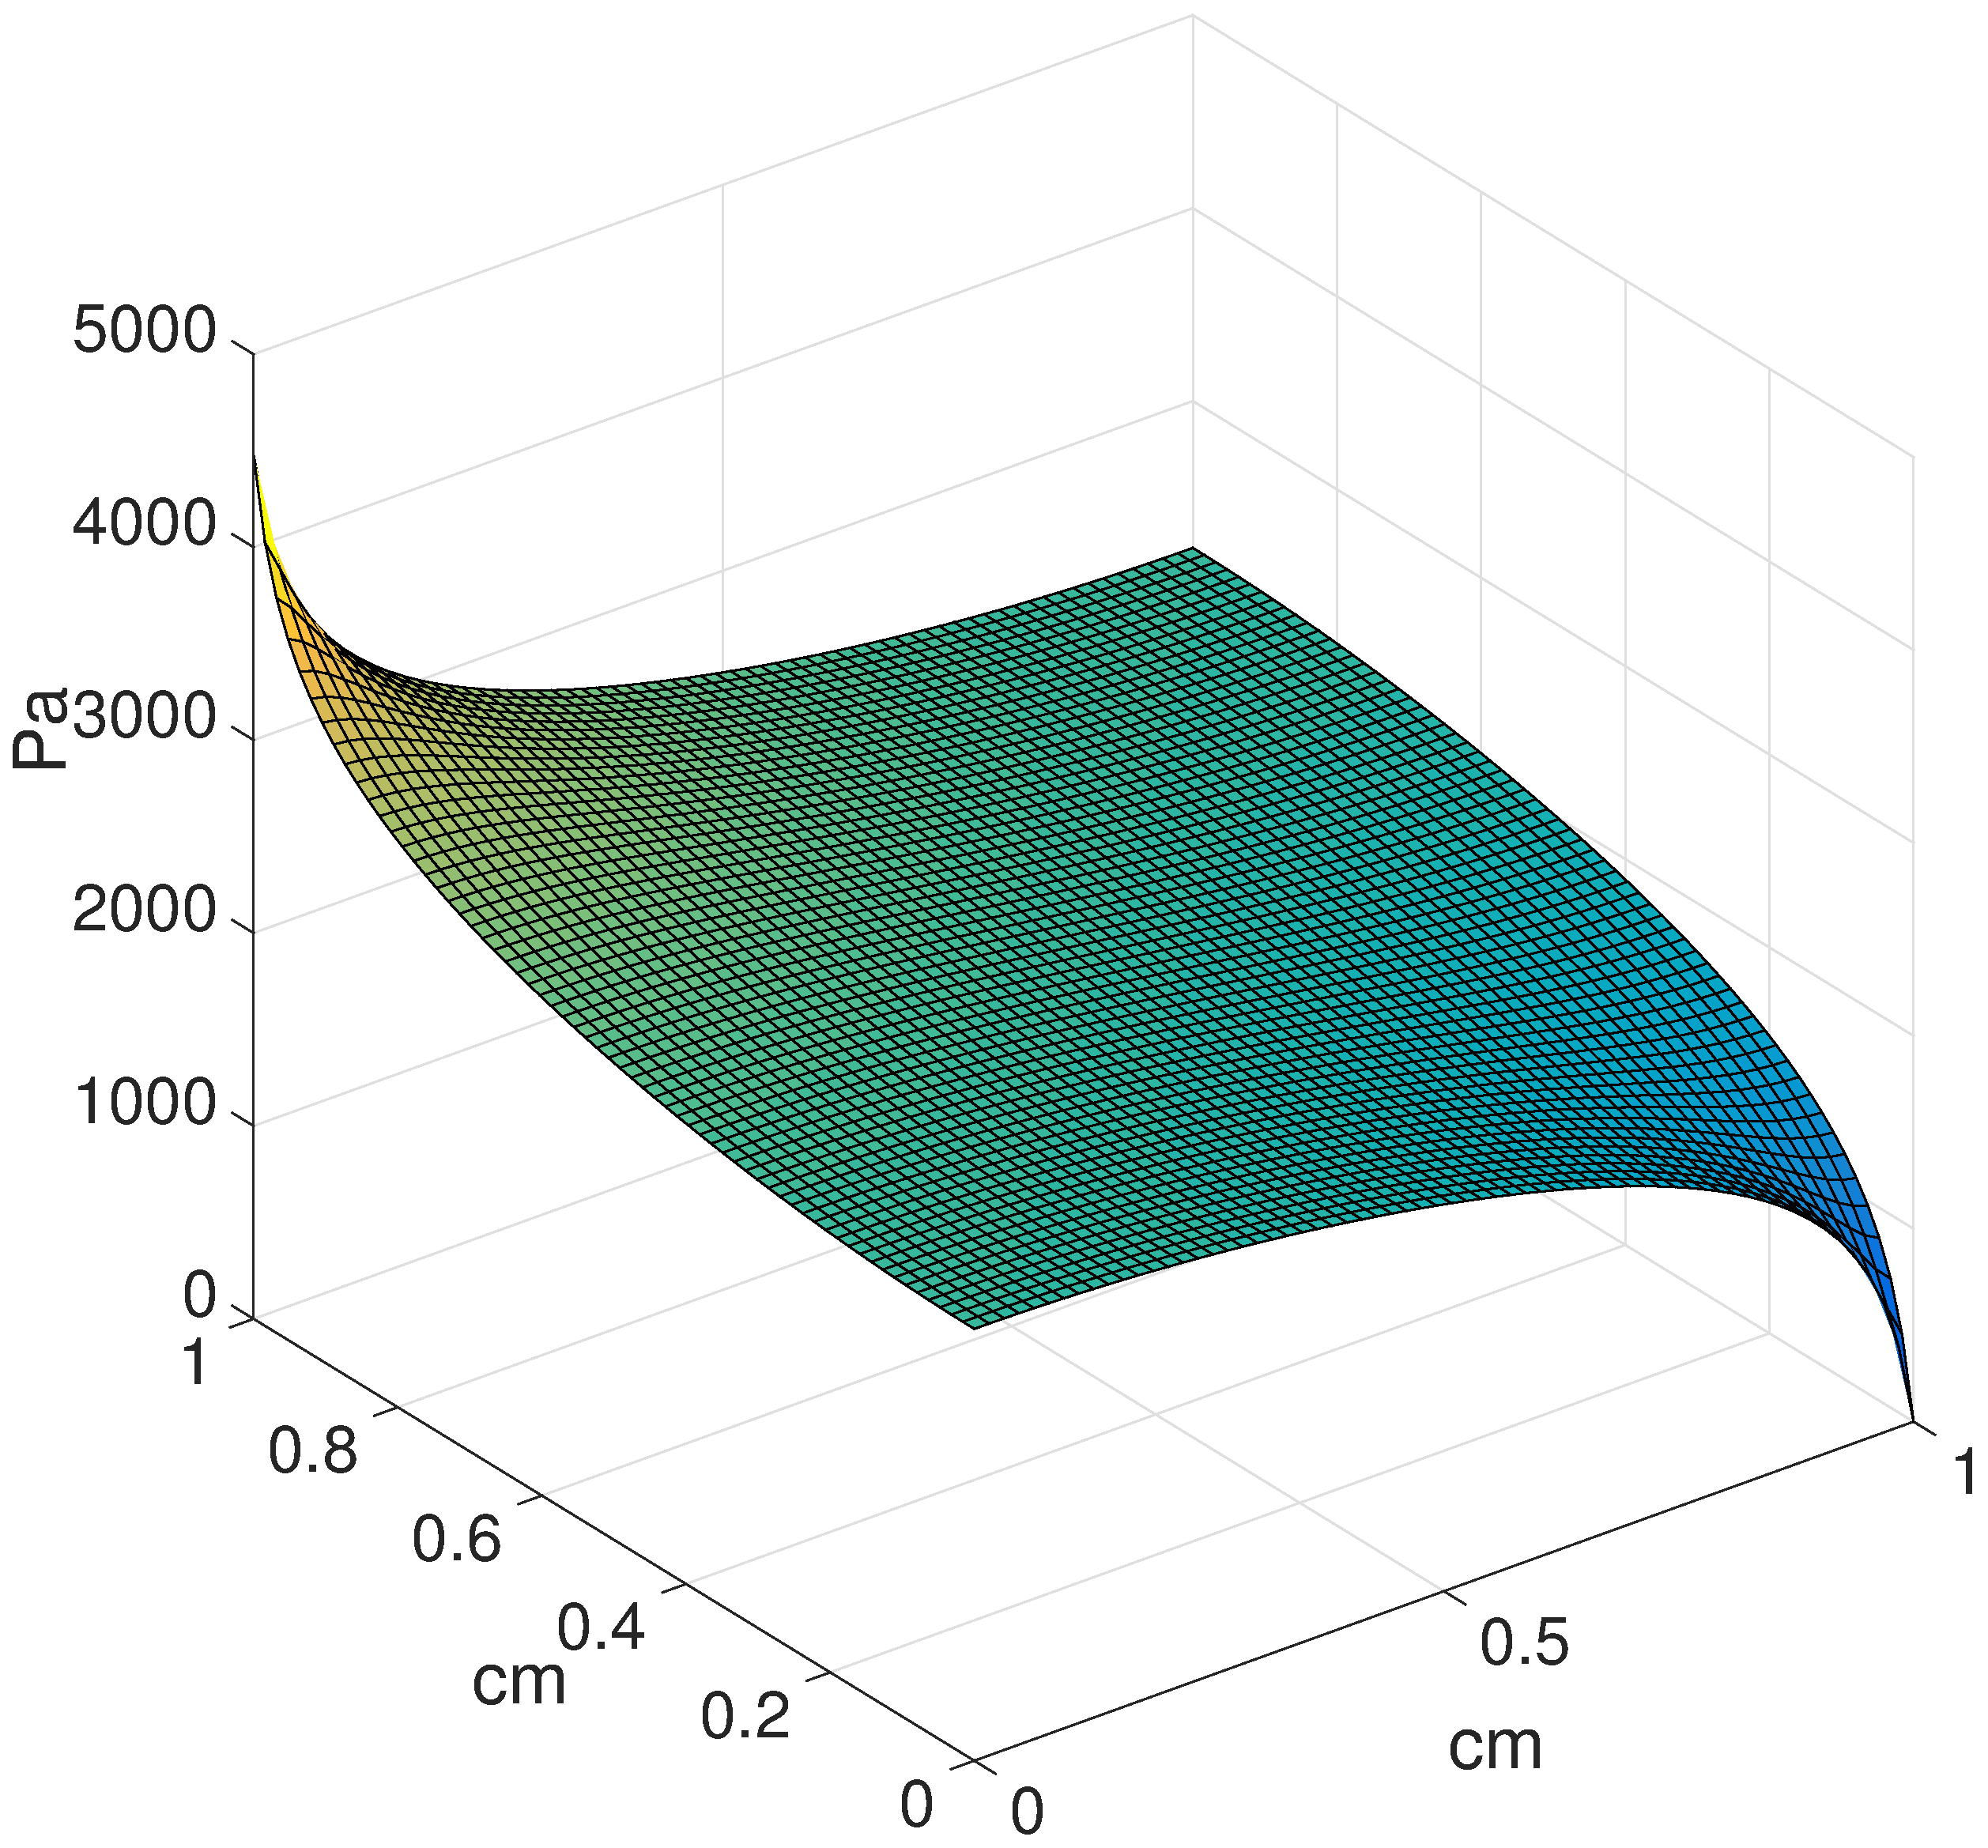
\includegraphics[width=\textwidth]{figs/pressure.eps}
                \caption{Pressure field $p$.}
            \end{subfigure} 
            \begin{subfigure}[b]{0.3\textwidth}
				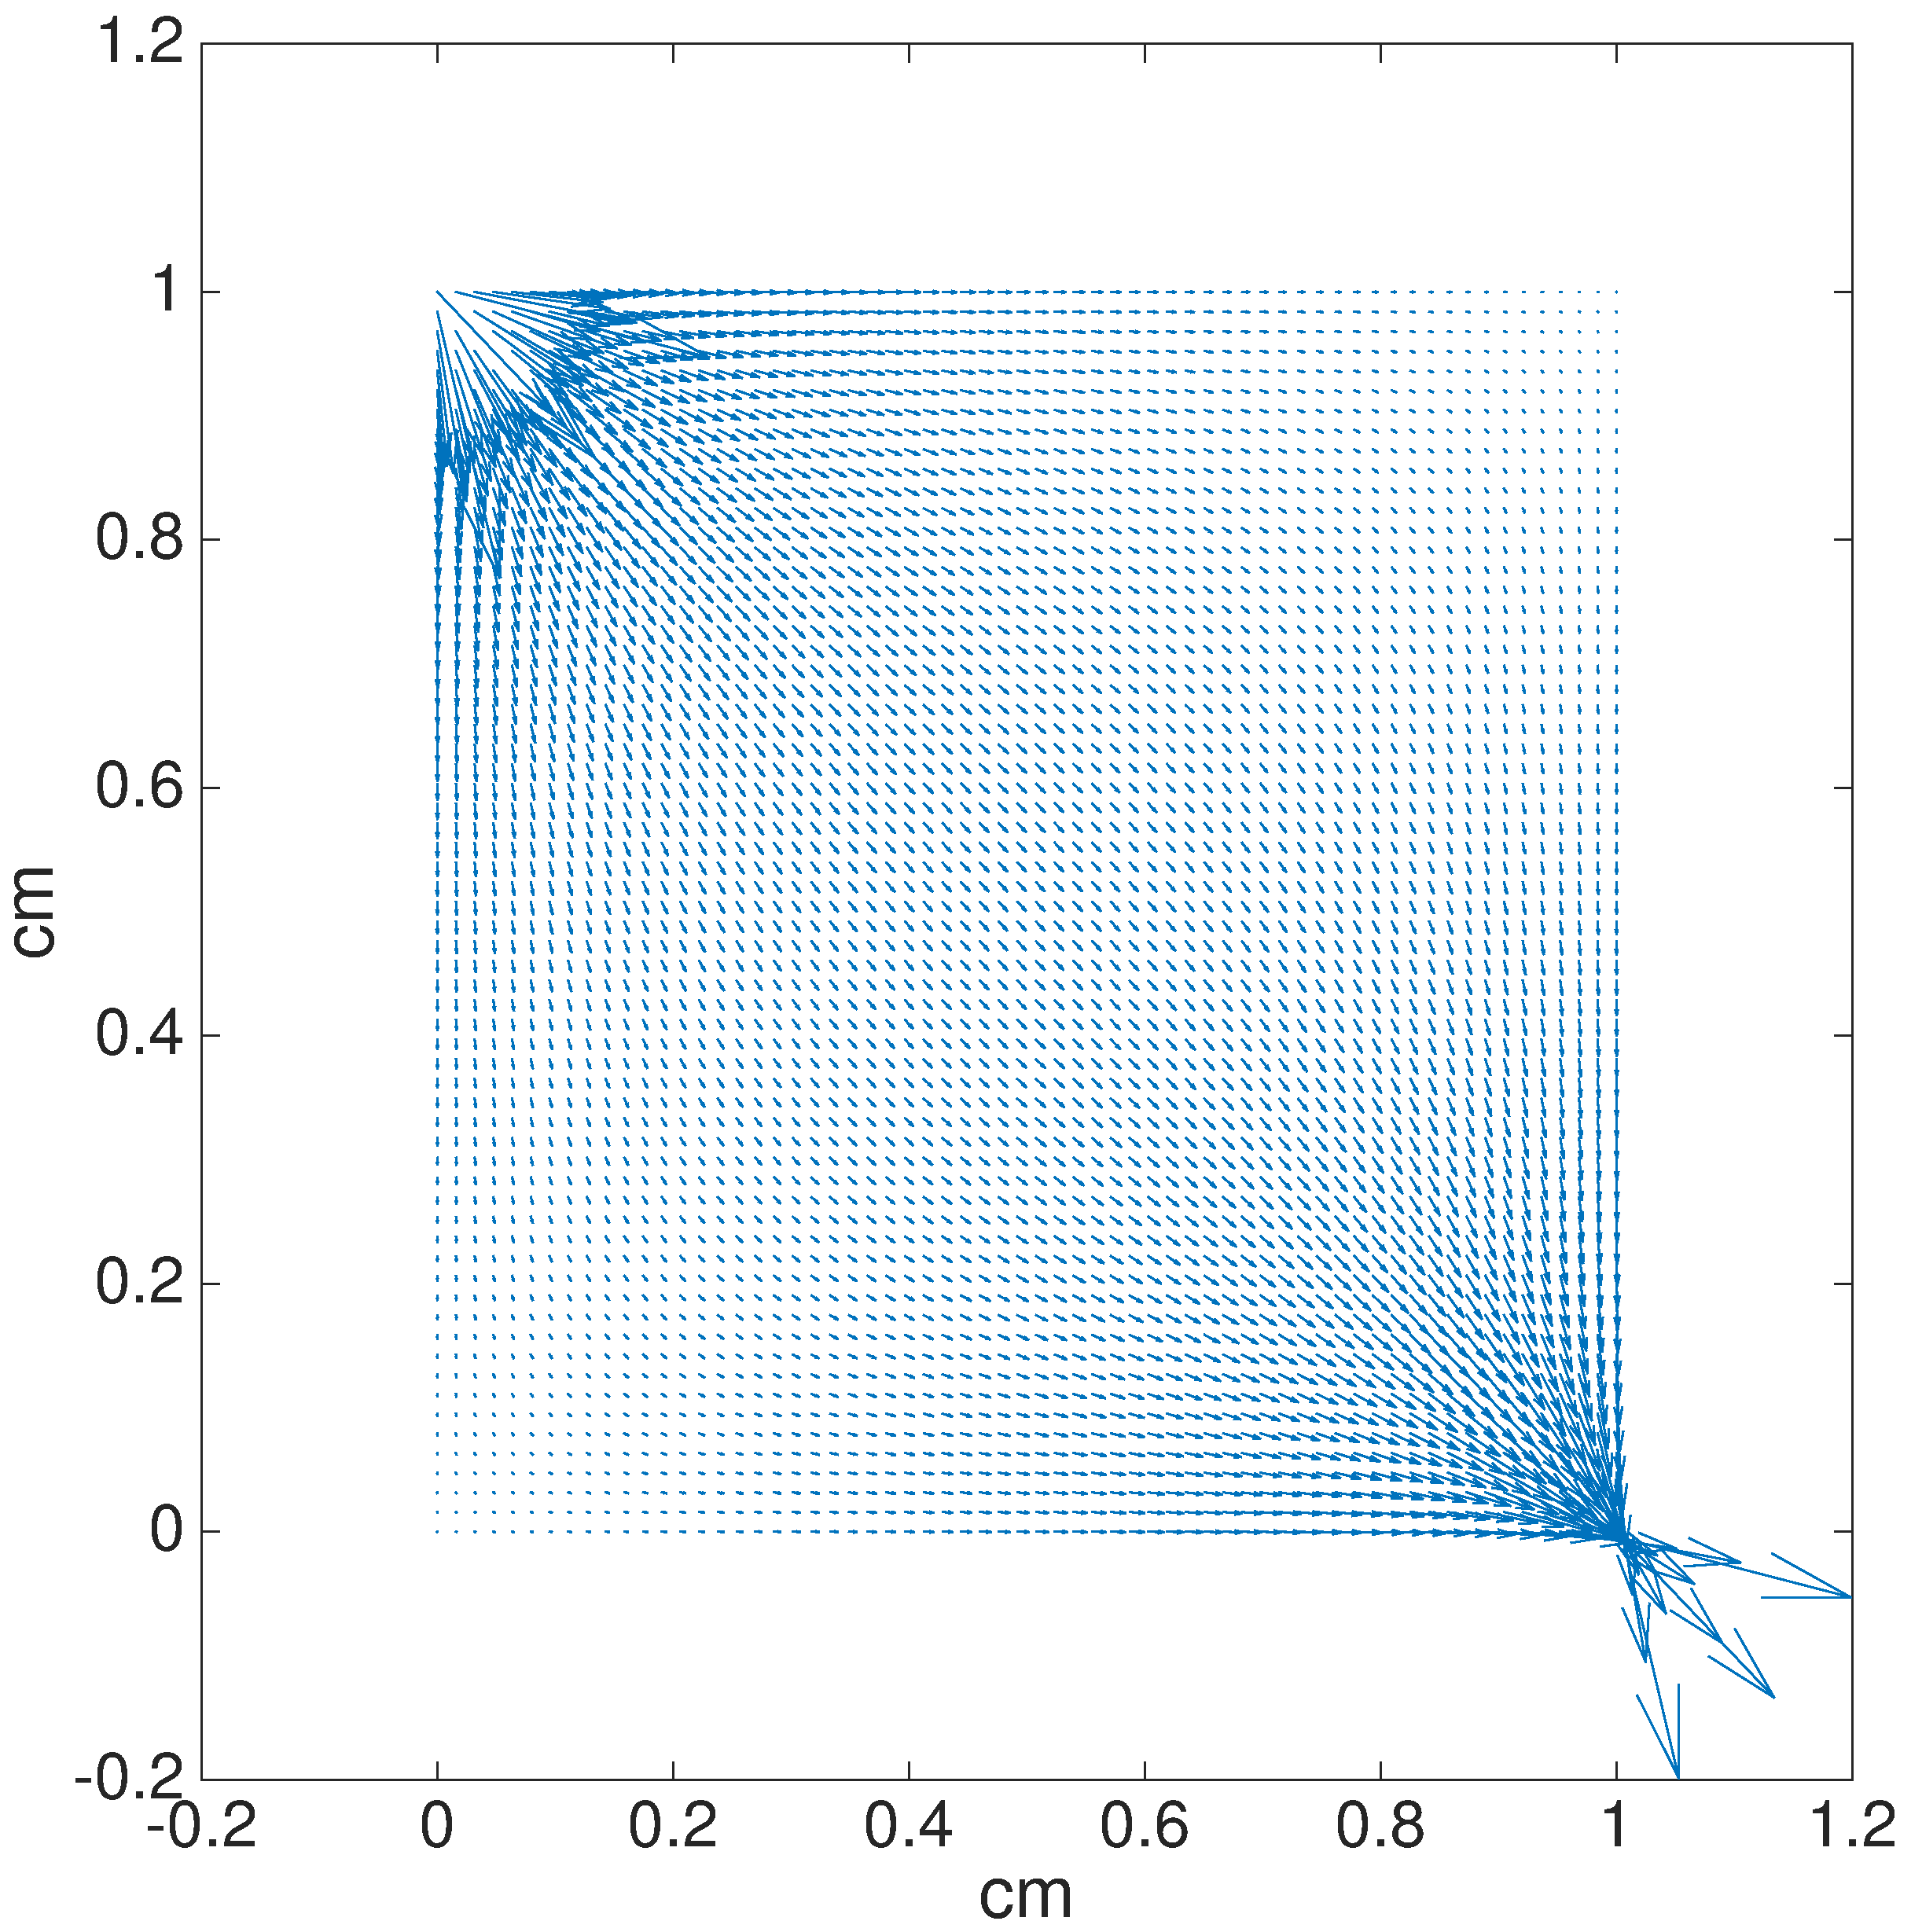
\includegraphics[width=\textwidth]{figs/flowQuiver.eps}
                \caption{Flow field $q$.}
            \end{subfigure}	           	                     
            \begin{subfigure}[b]{0.3\textwidth}
				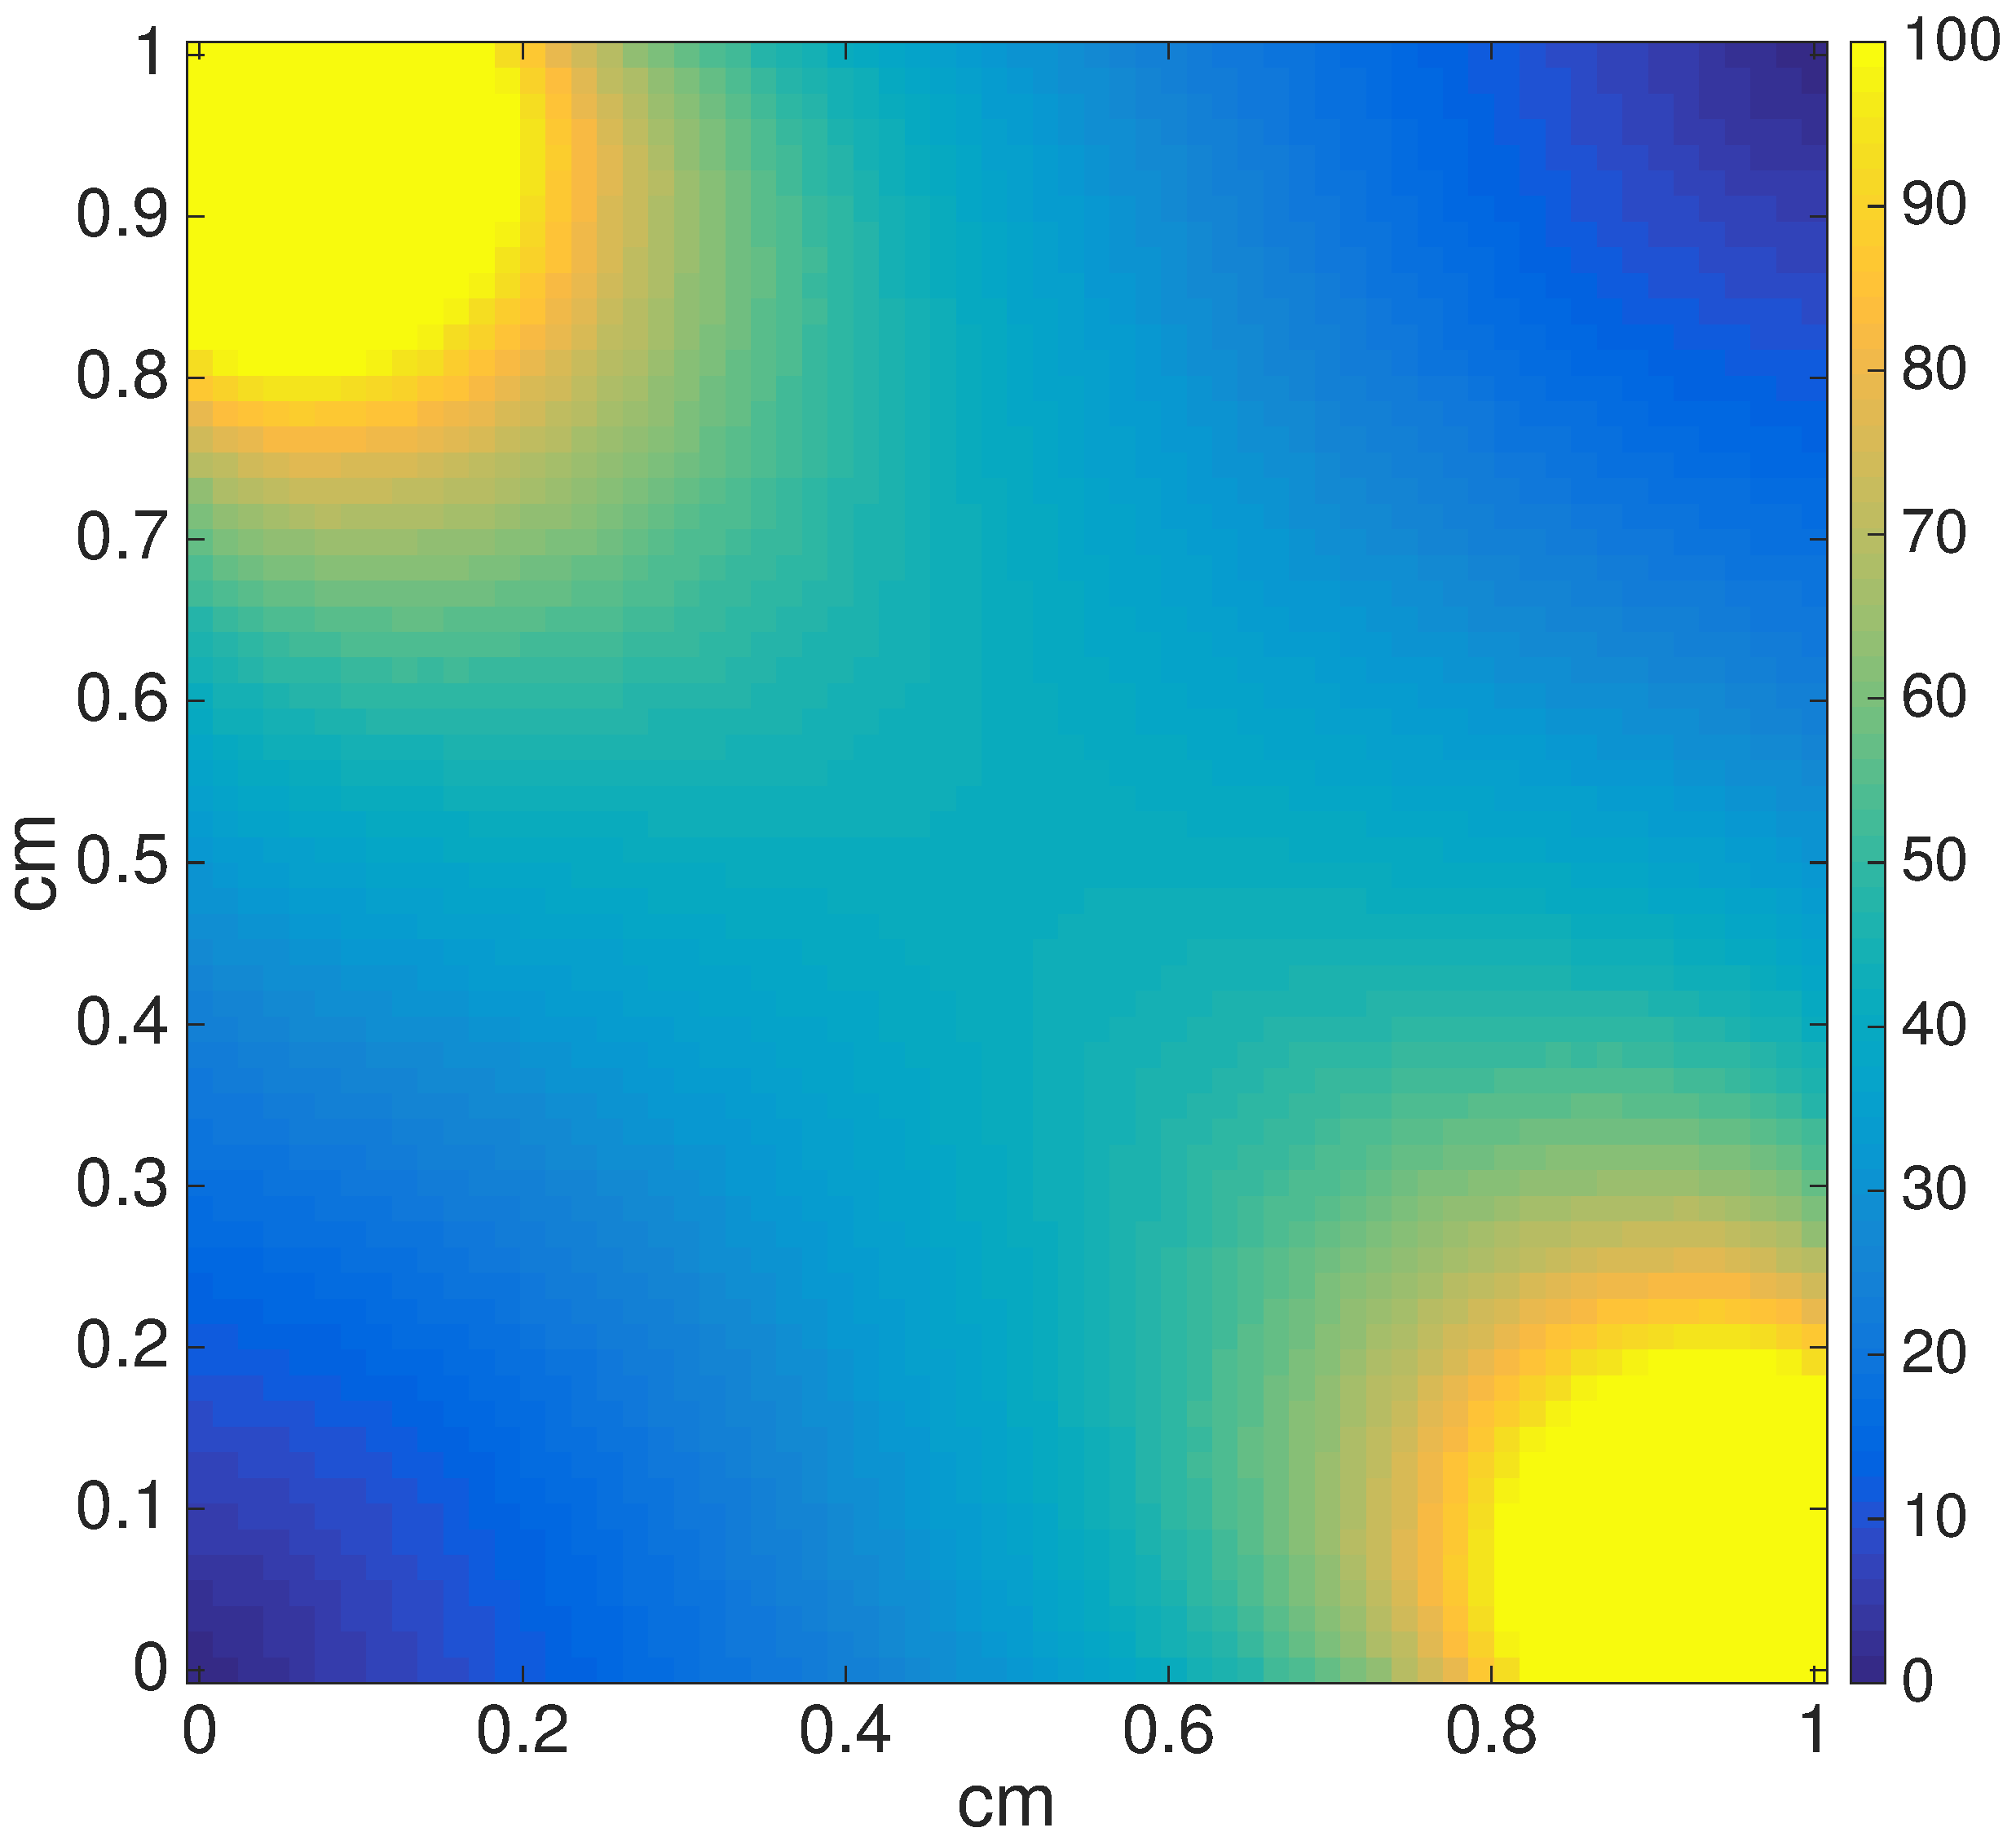
\includegraphics[width=\textwidth]{figs/perfusion.eps}
                \caption{Perfusion $P$.}
            \end{subfigure}	                
    	\caption{Synthetic flow model with a source in the upper left corner and a sink in the lower right corner. (a) Pressure field from solving the linear system in \eqref{eq:flowmodel}, in \si{\pascal} (b) flux field, (c) Voxelwise perfusion according to \eqref{eq:flux2perf} in \si{\siP}.}
	        \label{fig:flowpressureperfusion}
	\end{figure}
	
	\begin{figure}[H]
		\centering
		\begin{subfigure}[b]{0.45\textwidth}
			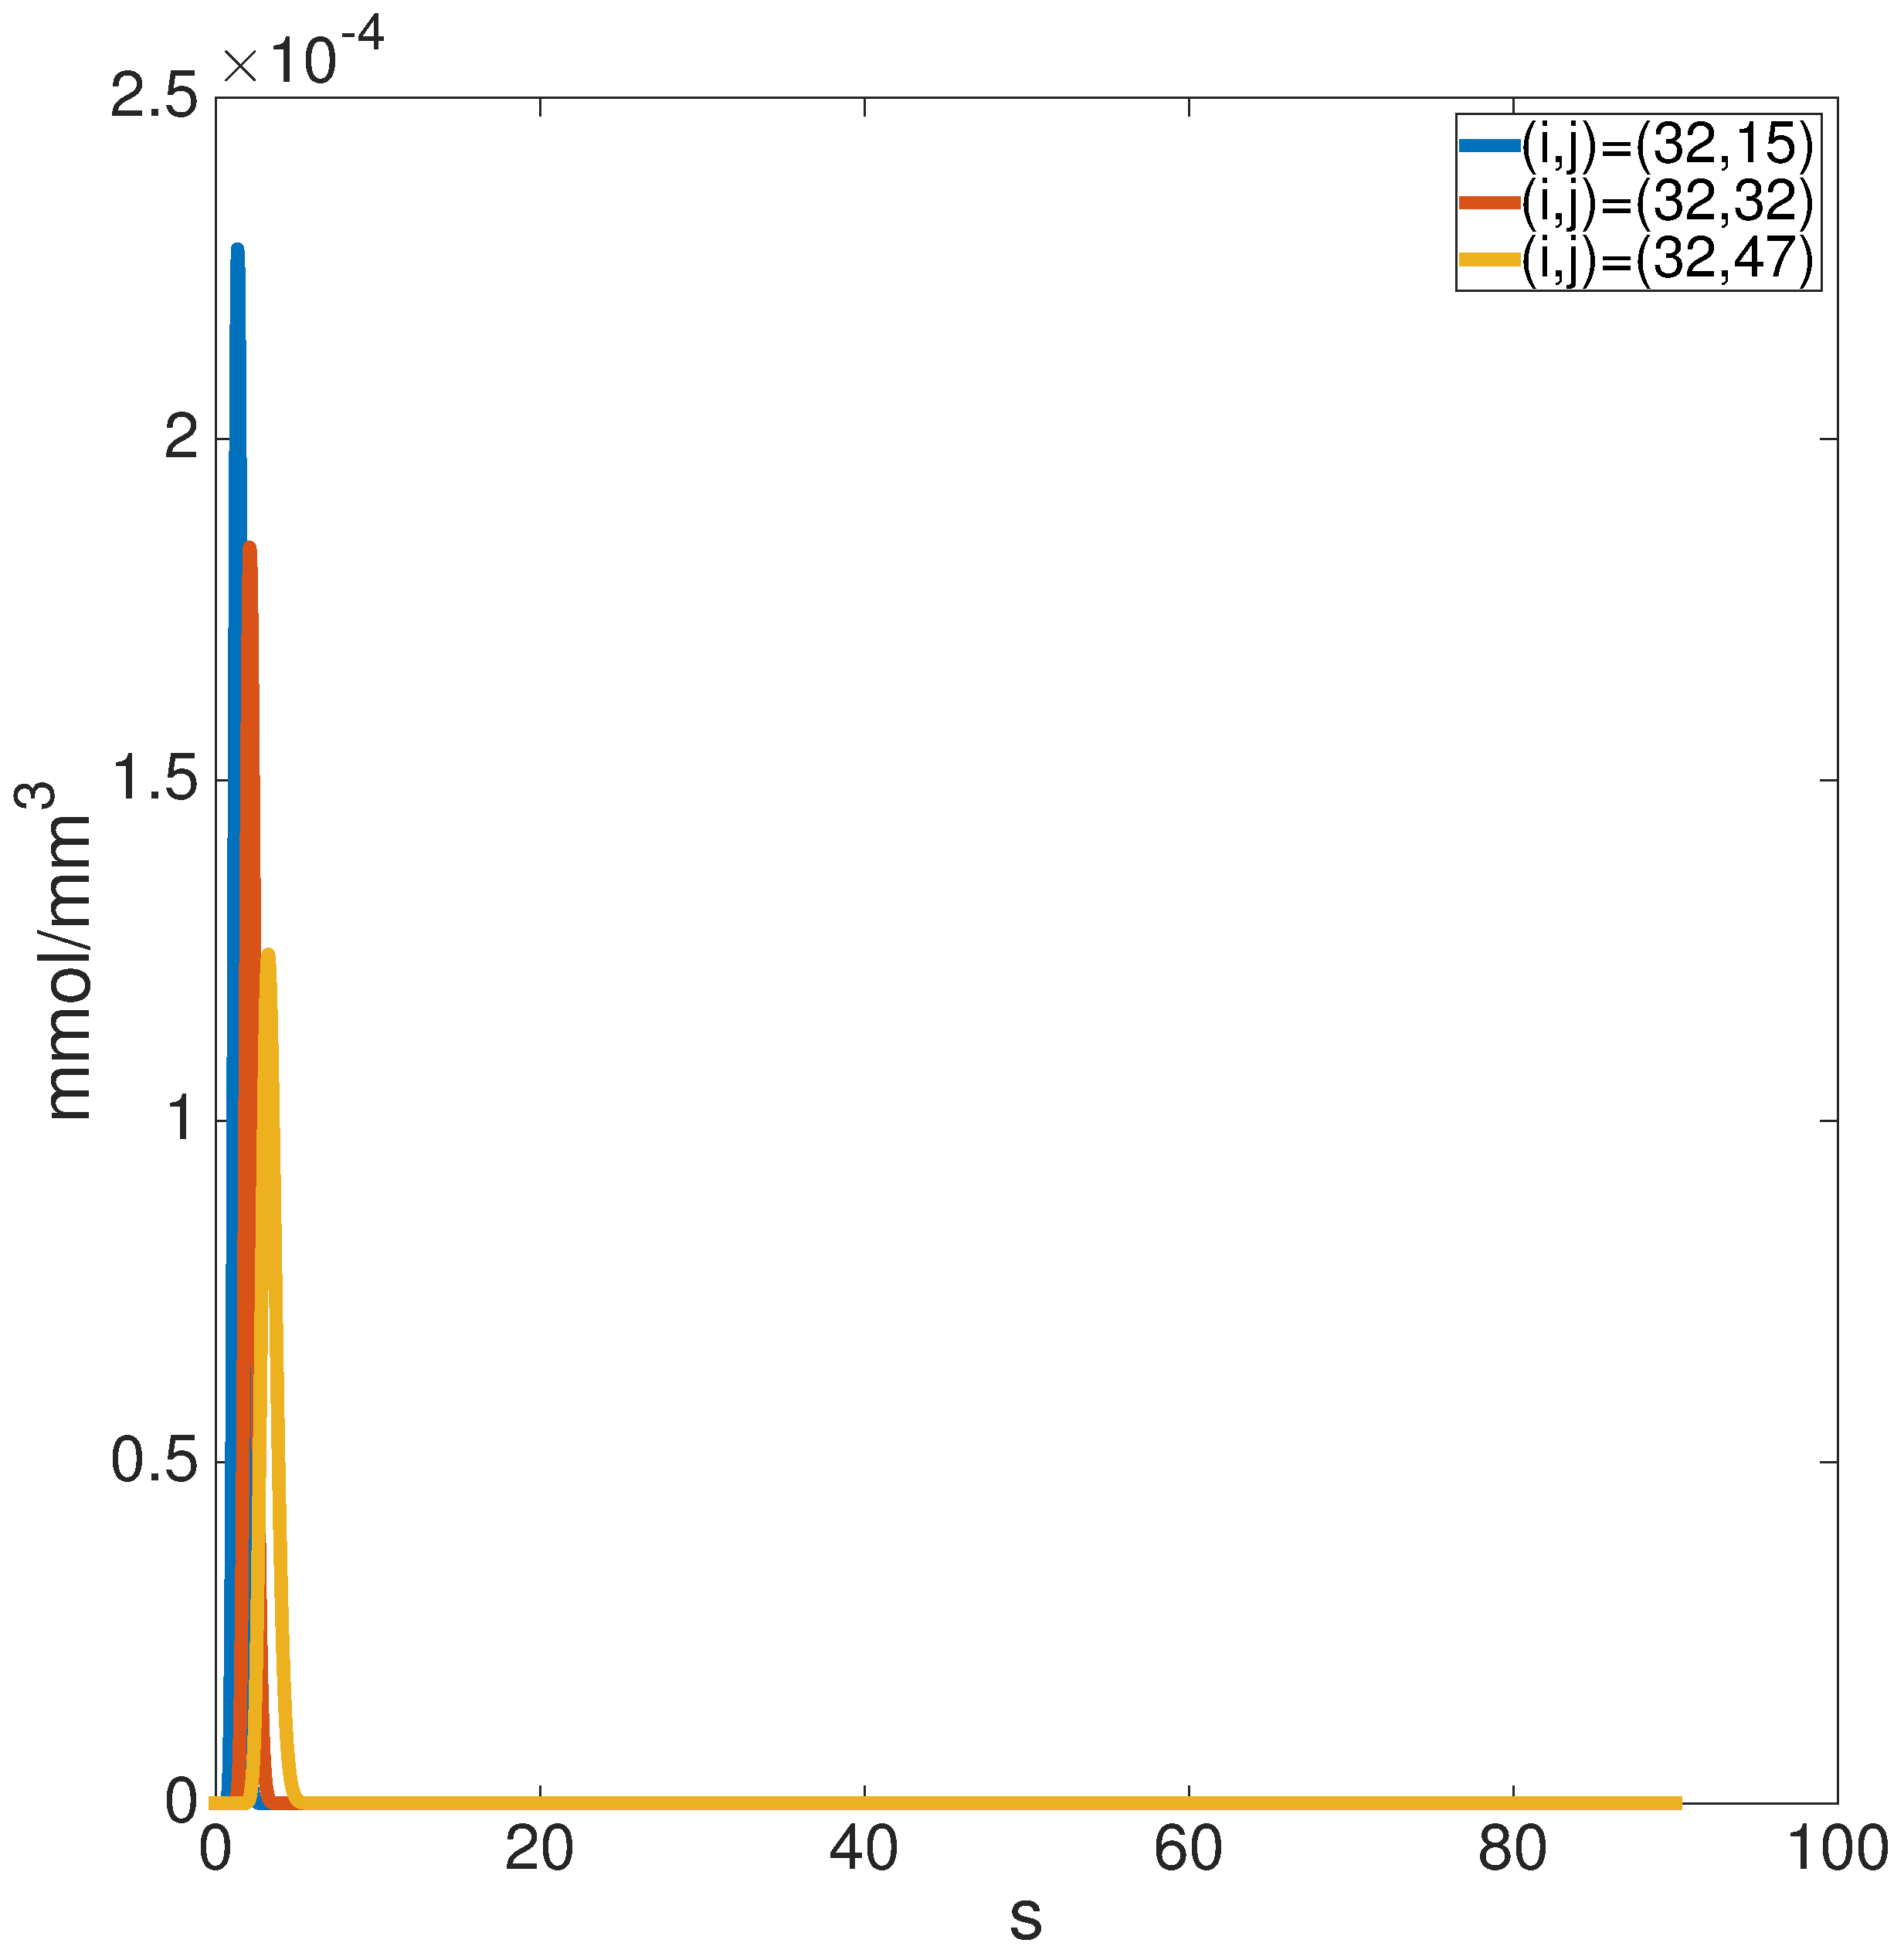
\includegraphics[width=\textwidth]{figs/PM153247.eps}
			\caption{Porous Media Model}
		\end{subfigure}
		\begin{subfigure}[b]{0.45\textwidth}
			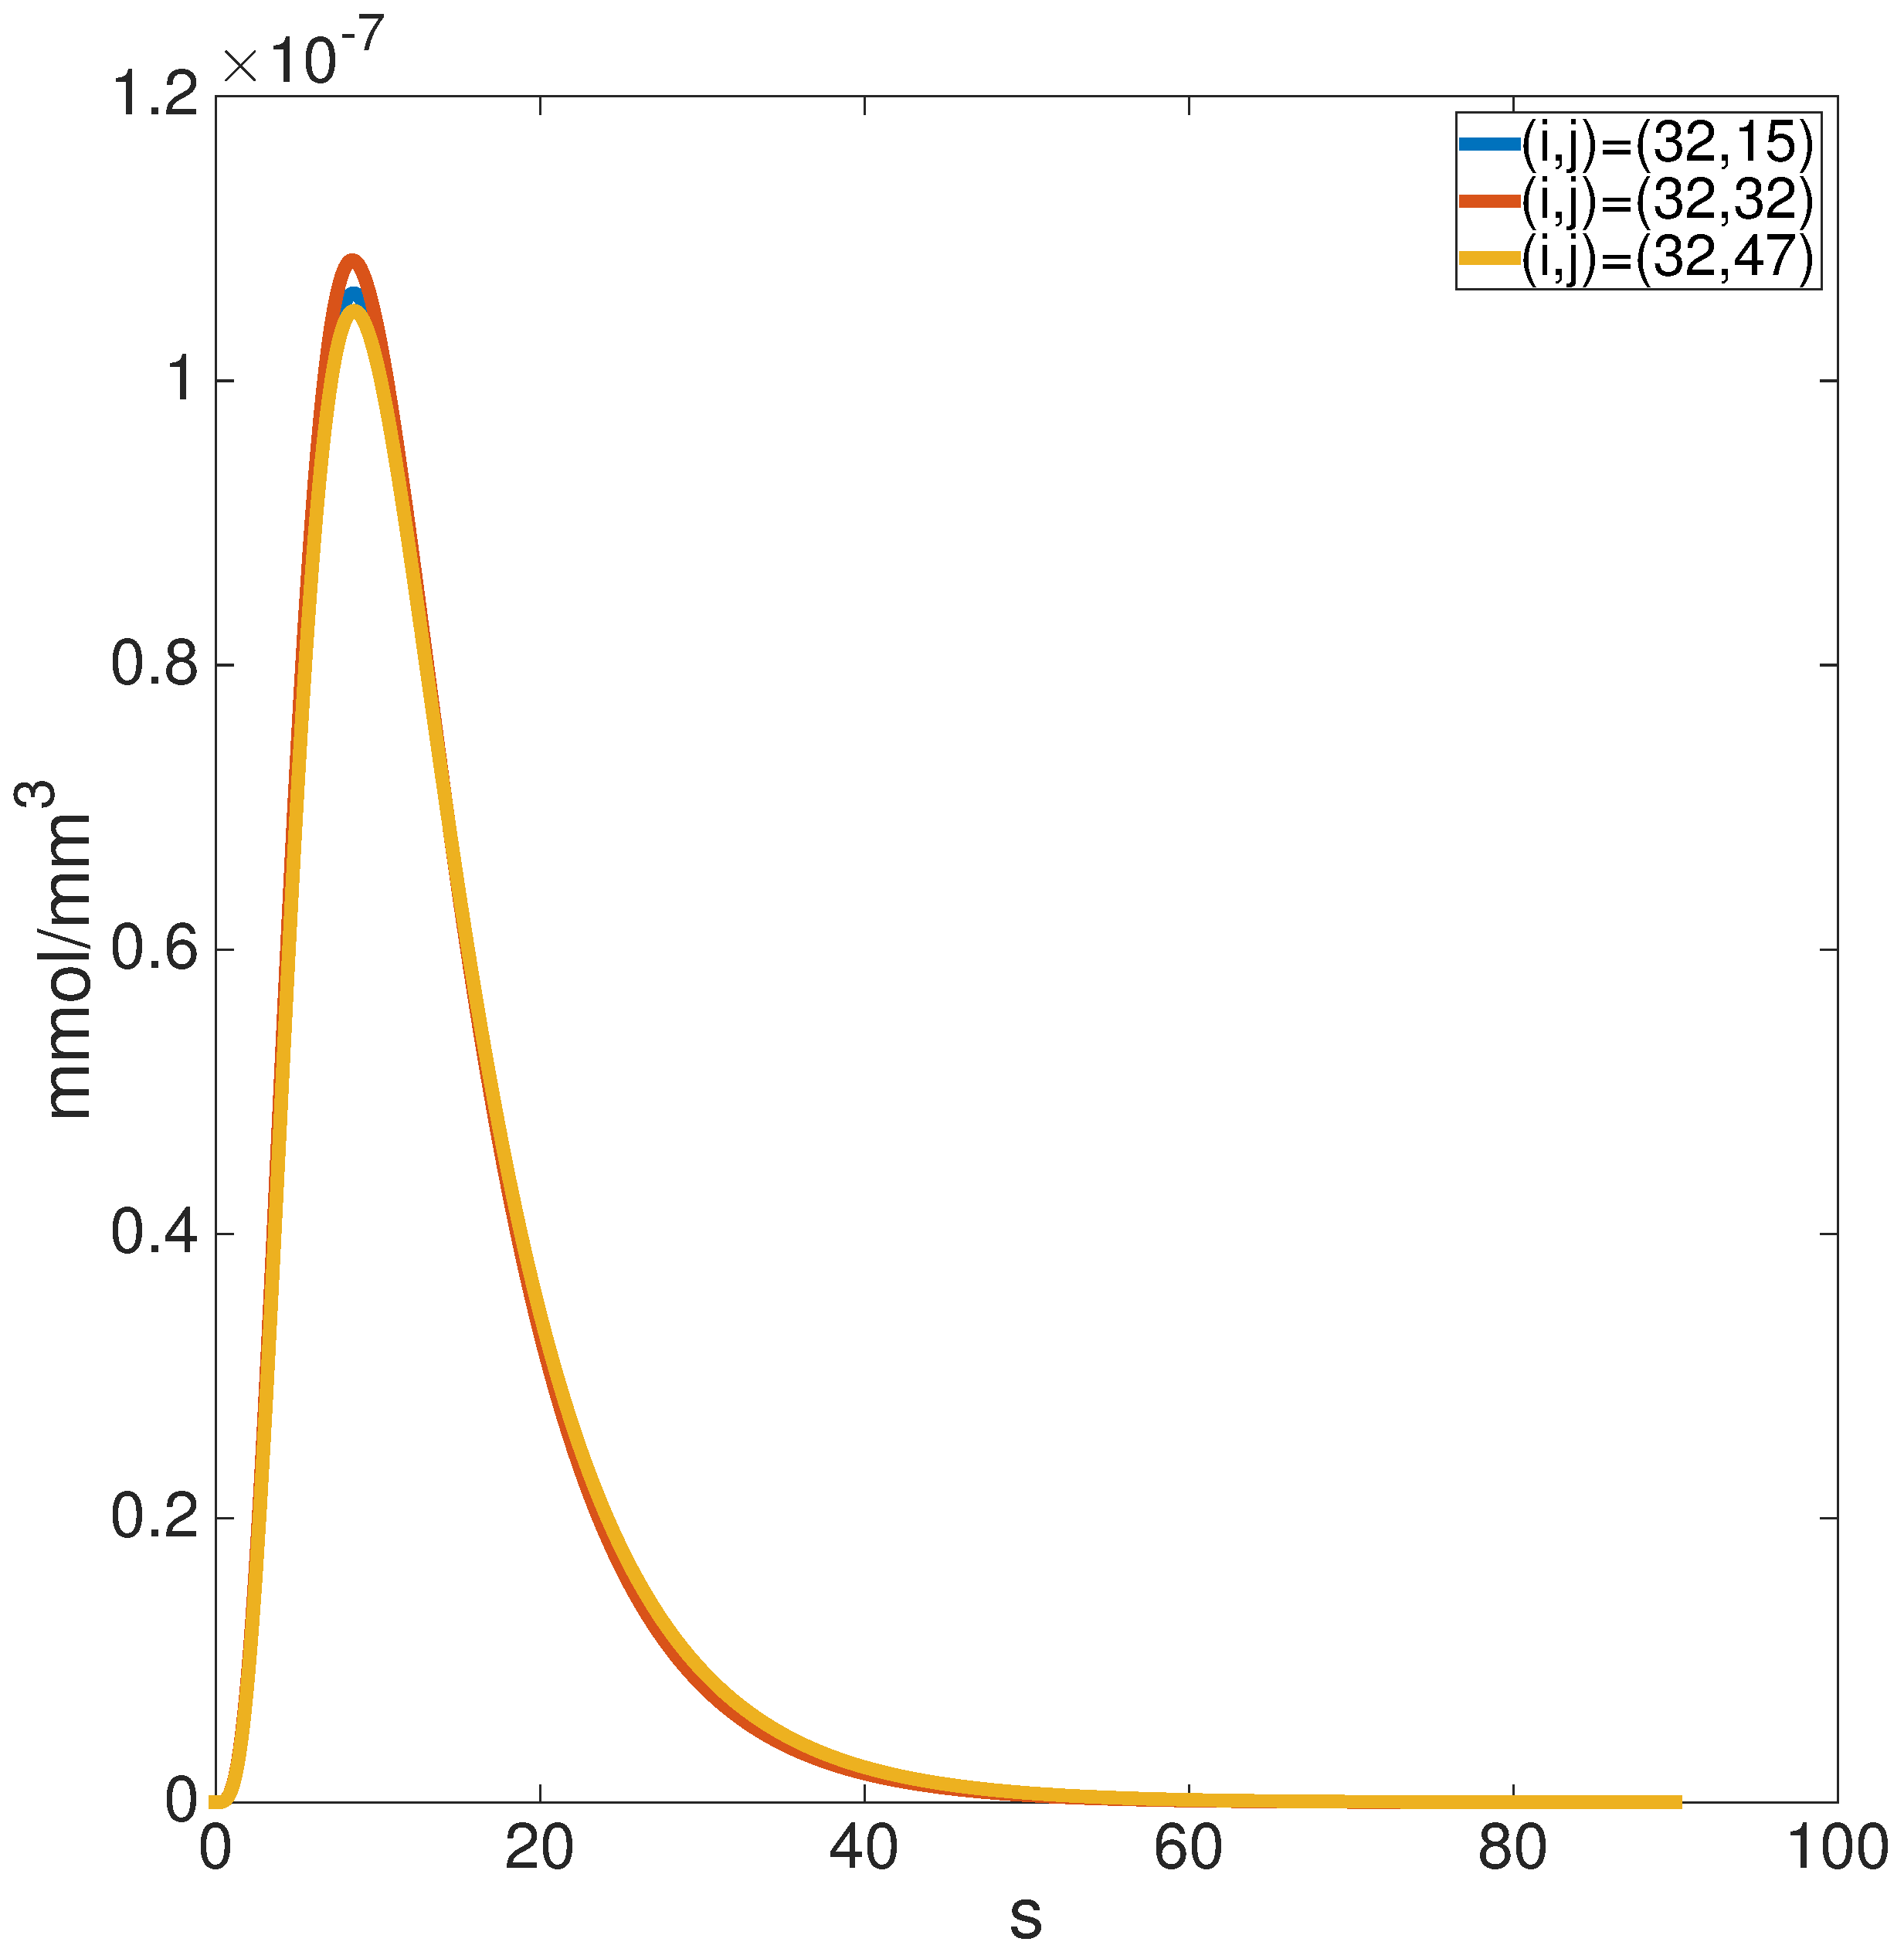
\includegraphics[width=\textwidth]{figs/RM153247.eps}			
			\caption{Reference Model}			
		\end{subfigure}		
		\caption{Comparison of tissue curves in the Porous Media (a) and the Reference Model (b). Curves were sampled in the middle row $i=32$ and columns $j \in \{15,32,47\}$.}
		\label{fig:tissuecomp}
	\end{figure}
	
	

	%--------------------------------------------------
	%--------------------------------------------------
	% Section: Results
	%--------------------------------------------------
	%--------------------------------------------------
	\section{Results}\label{sec:results}

	We tested the the convolution based classical model \eqref{eq:conv} as well as maximum-slope model \eqref{eq:MS} for their capability to recover the perfusion values.
	The success of the restoration was measured voxelwise in terms of the relative error of the recovered perfusion with respect to the true perfusion
	\[
		RE := \frac{\vert P_{\mathrm rec} - P_{\mathrm true}\vert}{P_{\mathrm true}}\cdot 100\%.
	\]
	Prior to reconstruction, the input data was downsampled to a time-resolution of $\SI{1}{\second}$.
	In order to simulate different spatial resolutions of the scanning process, the data was averaged using different block-sizes ranging from $(1,1)$ to $(64,64)$.
	Results are displayed in Figure \ref{fig:resultsPMM} as well as in Table \ref{tab:resultsSim}.
	
	\begin{table}[H]
		\caption{Results of the perfusion restoration with median relative errors in percent. Relative error was computed block-wise as $\vert P_{\mathrm rec} - P_{\mathrm true}\vert / P_{\mathrm true}\cdot 100\%$. Displayed is the median RE over the entire domain.}
		\centering
		\begin{tabular}{l c c c c c }
			& Model & \multicolumn{4}{c}{Block Size}\\
			 					 			& 		& (1,1) 	& (5,5)		& (10,10)	& entire domain \\
			\toprule
			\multirow{2}{*}{PMM: Perfusion} & MS 	& $170.09$ 	& $165.03$ 	& $158.57$	& $2.65$ \\
			 					 	   		& bSVD  & $859.06$ 	& $768.58$ 	& $664.84$	& $1.25$ \\
			\multirow{2}{*}{RM: Perfusion} & MS 	& $23.20$ 	& $24.26$ 	& $25.75$ 	& $37.96$ \\
			 					 			& bSVD  & $2.43$ 	& $4.27$ 	& $8.80$ 	& $20.72$ \\
			\midrule											
			PMM: CBV & & $4.37\cdot10^{-5}$      & $4.37\cdot10^{-5}$		& $4.37\cdot10^{-5}$		& $4.37\cdot10^{-5}$ \\											
			RM:  CBV & & $1.94\cdot10^{-2}$      & $1.93\cdot10^{-2}$		& $2.12\cdot10^{-2}$		& $1.13$ 			
		\end{tabular}
		\label{tab:resultsSim}
	\end{table}
	
	
	It can be seen that for the complete domain the perfusion can be accurately restored by both methods with an error of ca. $2\%$.
	However, for the voxel-wise model the classic method works not as expected.
	Impuls response function reconstructed from the Porous Media Model are displayed in Figure \ref{fig:deconvResults}.
	These are clearly not exhibiting the properties described in Section \ref{sec:conv}.
	This is possible due to the reason that the model assumptions of \eqref{eq:conv} are violated \todo{CH: Let me think about this a bit harder...}.
	Also dispersion effects might be playing a role \cite{calamante03}. 
	However, these effects are typically leading to underestimation of perfusion, the opposite of the drastic overestimation the data is showing.	



	\newcommand{\inc}[1]{\includegraphics[width = .25\textwidth]{./figs/#1}}
	\newcommand{\rbox}[2]{\rotatebox{90}{\hspace{#1}\mbox{\large #2}}}
	\begin{figure}[H]
		\centering
		\begin{tabular}{c c c c}
			 \rbox{0ex}{True perfusion} & \inc{recTrue-1.eps} & \inc{recTrue-5.eps} & \inc{recTrue-10.eps}\\
			 \rbox{5ex}{bSVD} & \inc{recCirc-PDE-1.eps} & \inc{recCirc-PDE-5.eps} & \inc{recCirc-PDE-10.eps}\\
			 \rbox{8ex}{MS} & \inc{recMS-PDE-1.eps} & \inc{recMS-PDE-5.eps} & \inc{recMS-PDE-10.eps}\\			 			 			  
			   & (1,1) & (5,5) & (10,10)
		\end{tabular}
		\caption{Results of the restoration of perfusion for the Porous Media Model (PMM) for different levels of discretization, displayed in the columns. All results are given in $\mathrm{ml/min/100ml}$. First Row: Ground-Truth Perfusion (cf. Section \ref{sec:flux2perf}). Second Row: Perfusion as estimated by bSVD. Third Row: Perfusion as estimated by the Maximum-Slope model.}	
		\label{fig:resultsPMM}			
	\end{figure}



	\begin{figure}[H]
		\centering
			\begin{tabular}{c c}
				 \inc{C-and-Crec.eps} & \inc{Irec.eps} \\
				 \multicolumn{2}{ c }{(a) Entire Domain, PMM} \\
				 \inc{C-and-Capprox-cap.eps} & \inc{IR-cap.eps} \\			 
				 \multicolumn{2}{ c }{(b) Inside the capillary bed, PMM} \\				 
				 \inc{C-and-Crec-conv.eps} & \inc{Irec-conv.eps} \\			 
				 \multicolumn{2}{ c }{(c) Inside the capillary bed, RM} \\				 				 
			\end{tabular}
		\caption{Results for the deconvolution model. First row: Results of bSVD applied to PMM with block-size (64,64) (i.e. entire domain) (Model-Fit and Impuls-Response Function). Second row: Results of bSVD applied to a single voxel of the PMM in the inside of the domain. Third row: Second row: Results of bSVD applied to a single voxel of the SCD in the inside of the domain.}			
		\label{fig:deconvResults}
	\end{figure}

	
	
	%--------------------------------------------------
	%--------------------------------------------------
	% Section: Conclusion
	%--------------------------------------------------
	%--------------------------------------------------	
	\section{Conclusion}\label{sec:conclusion}
	Missing
	
	%--------------------------------------------------
	% Bibliography
	%--------------------------------------------------
	\bibliographystyle{ieeetr}	
	\bibliography{./bibliography.bib}

	
\end{document}